\begin{mainquestion}{resistor_code}{Resistor Code}

Your good friend built the resistor network shown below on a breadboard but it didn’t perform as expected, and they’ve asked for your help. They’ve been making do with leftovers and have used quite a variety of resistors. You are without your trusty multimeter so you’ll have to do the best you can with a visual inspection.

\begin{figure}[htbp]
    \centering
    % Left Image (No Caption)
    \begin{minipage}[b]{0.45\textwidth}
        \centering
        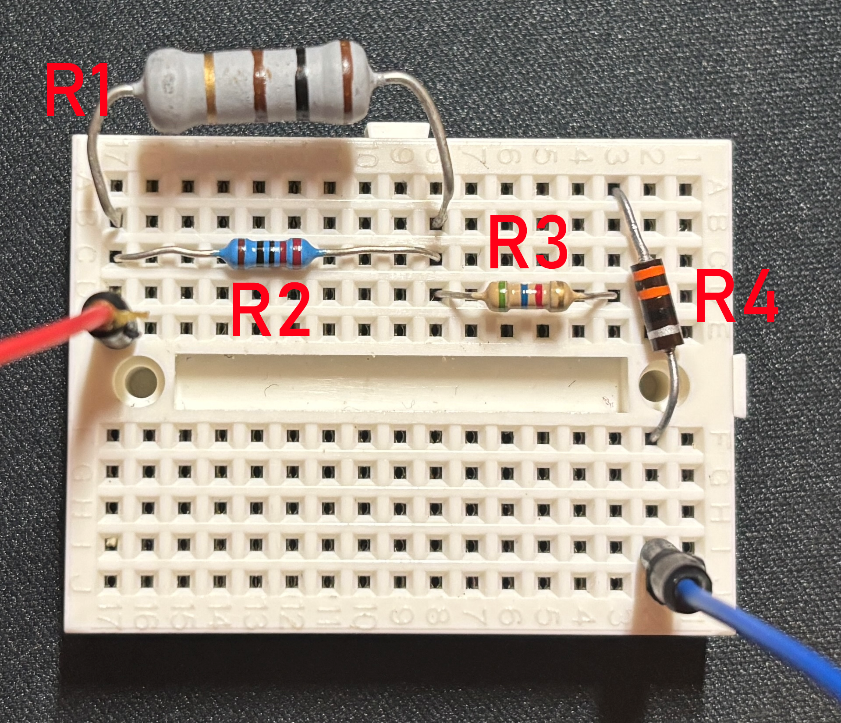
\includegraphics[width=\textwidth]{circuit.png}
    \end{minipage}
    \hfill % Adds horizontal space between the two images
    % Right Image (With Caption)
    \begin{minipage}[b]{0.45\textwidth}
        \centering
        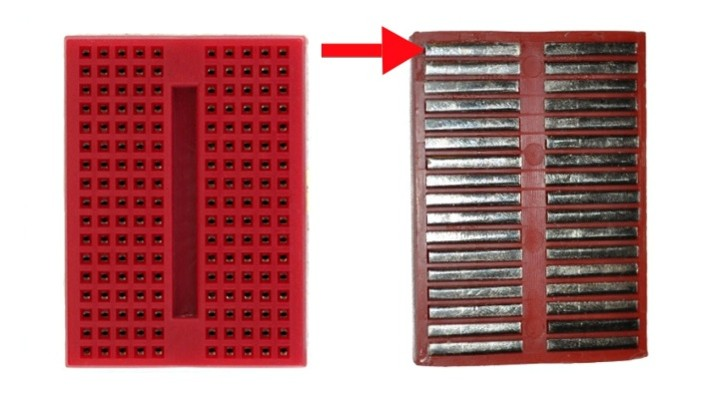
\includegraphics[width=\textwidth]{breadboard.jpg}
        \caption{Sparkfun Mini Breadboard Wiring Diagram}
        \label{fig:breadboard}
    \end{minipage}
\end{figure}

\textit{For clarity, the colored stripes are listed below as they appear in the image. Reference the image and the resistor color code chart to sort out the direction the stripes should be read.}

\begin{table}[htbp]
    \centering
    \label{tab:resistor_codes}
    \begin{tabular}{l l l l l l l}
        \hline
        \textbf{Resistor} & \textbf{Direction} & \textbf{Band A} & \textbf{Band B} & \textbf{Band C} & \textbf{Band D} & \textbf{Band E} \\ 
        \hline
        R1 & Left to right & Gold   & Brown  & Black & Brown  & --- \\
        R2 & Left to right & Brown  & Black  & Black & Red    & Red \\
        R3 & Left to right & Green  & Blue   & Red   & Gold   & --- \\
        R4 & Top to bottom & Orange & Orange & Black & Silver & --- \\ 
        \hline
    \end{tabular}
\end{table}


% =========================================================
\begin{partquestion}{schematic}
{Given the photo of your friend’s circuit, draw a circuit diagram showing how the resistors are connected. Label your resistors with appropriate identifiers (R1, R2 …), resistor values, and tolerances.}

\begin{answer}
These resistors come from a variety of generations and technologies, but the color codes are still valid for all of them.

R1 -- Stripes read [Gold, Brown, Black, Brown]. The last band is typically separated from the others slightly, so we instead read this as [Brown, Black, Brown, Gold]. This indicates a resistance value of
\[
\num{10e1}=\qty{100}{\ohm}\pm\qty{5}{\percent}.
\]
It is also quite large, so we expect the power handling to be larger than the others.

R2 -- Stripes read [Brown, Black, Black, Red, Red]. As before, the brown band is separated, so we flip the sequence to [Red, Red, Black, Black, Brown]. This indicates
\[
\num{220e0}=\qty{220}{\ohm}\pm\qty{1}{\percent}.
\]

R3 -- Stripes read [Green, Blue, Red, Gold]. Gold is the tolerance band. This gives
\[
\num{56e2}=\qty{5.6}{\kilo\ohm}\pm\qty{5}{\percent}.
\]

R4 -- Stripes read [Orange, Orange, Black, Silver]. Silver is the tolerance band. This gives
\[
\num{33e0}=\qty{33}{\ohm}\pm\qty{10}{\percent}.
\]

\begin{center}    
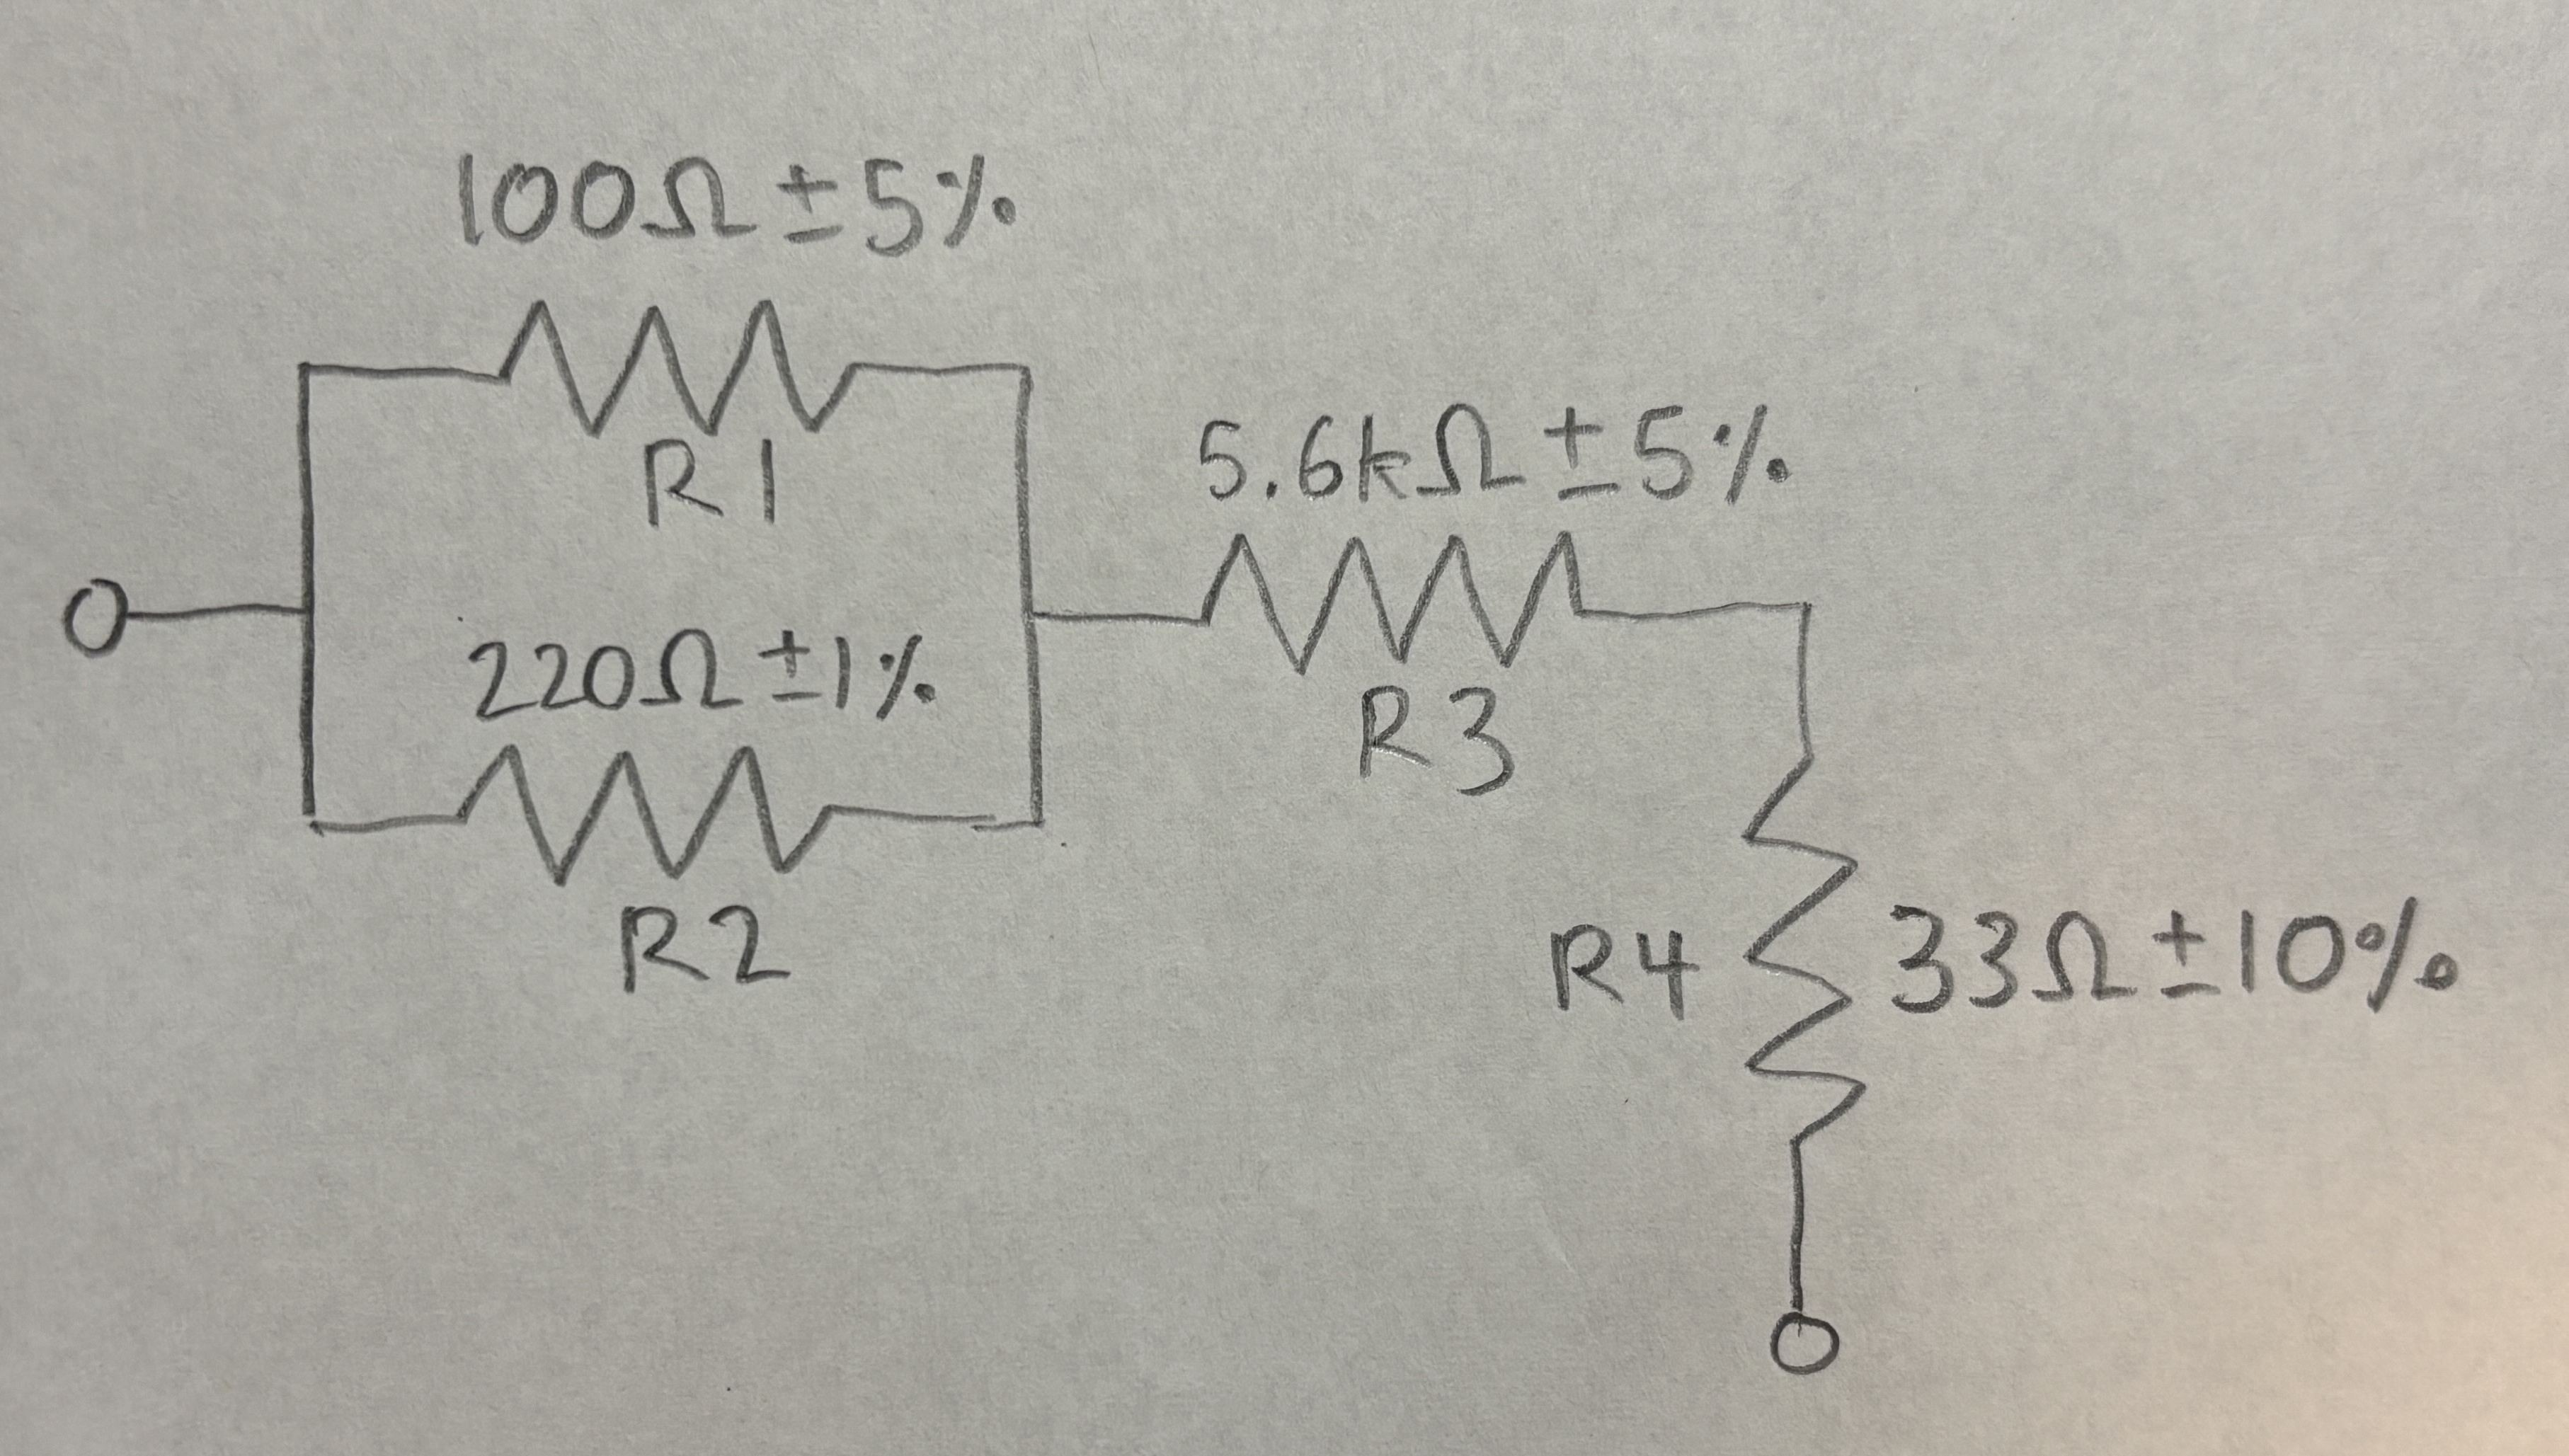
\includegraphics[width=0.8\textwidth]{schematic_sol.jpg}
\end{center}

\end{answer}
\end{partquestion}

% =========================================================
\begin{partquestion}{minmax}
{Your friend is concerned that this circuit may be sensitive to errors in resistance. What are the maximum and minimum expected values for R1 and R2?}

\begin{answer}

R1 has a tolerance of \qty{5}{\percent}:
\begin{align*}
R_{1,\min} &= \qty{100}{\ohm}\left(1-\num{0.05}\right) = \qty{95}{\ohm} \\
R_{1,\max} &= \qty{100}{\ohm}\left(1+\num{0.05}\right) = \qty{105}{\ohm}
\end{align*}

R2 has a tolerance of \qty{1}{\percent}:
\begin{align*}
R_{2,\min} &= \qty{220}{\ohm}\left(1-\num{0.01}\right) = \qty{218}{\ohm} \\
R_{2,\max} &= \qty{220}{\ohm}\left(1+\num{0.01}\right) = \qty{222}{\ohm}
\end{align*}

\end{answer}
\end{partquestion}

% =========================================================
\begin{partquestion}{temprange}
{Next your friend tells you that this circuit will be operating at an ambient temperature from \qty{-20}{\celsius} to \qty{60}{\celsius}. Suppose these resistors are specified at \qty{25}{\celsius} and have a TCR of $+300\text{ppm}/\qty{}{\celsius}$ and $-100\text{ppm}/\qty{}{\celsius}$ respectively, what are the maximum and minimum expected resistances they could have?}

\begin{answer}

Since the resistors are specified at \qty{25}{\celsius}, the temperature excursion is
\[
\Delta T_{\min} = \qty{-45}{\celsius}, \quad
\Delta T_{\max} = \qty{35}{\celsius}.
\]

The resistance variation is
\[
R = R_0\left(1 + \mathrm{TCR}\,\Delta T\right).
\]

R1 (positive TCR):
\begin{align*}
R_{1,\min} &= \qty{100}{\ohm}\left(1-\num{0.05}\right)\left(1+\num{300e-6}\cdot\num{-45}\right)
= \qty{93.7}{\ohm} \\
R_{1,\max} &= \qty{100}{\ohm}\left(1+\num{0.05}\right)\left(1+\num{300e-6}\cdot\num{35}\right)
= \qty{106.1}{\ohm}
\end{align*}

R2 (negative TCR):
\begin{align*}
R_{2,\min} &= \qty{220}{\ohm}\left(1-\num{0.01}\right)\left(1-\num{100e-6}\cdot\num{35}\right)
= \qty{217.0}{\ohm} \\
R_{2,\max} &= \qty{220}{\ohm}\left(1+\num{0.01}\right)\left(1-\num{100e-6}\cdot\num{-45}\right)
= \qty{223.2}{\ohm}
\end{align*}

\end{answer}
\end{partquestion}

% =========================================================
\begin{partquestion}{colorswitch}
{After reviewing your schematic, your friend realizes that R3 is 10 times smaller than intended. What is the correct color code?}

\begin{answer}
R3 was [Green, Blue, Red, Gold], corresponding to \qty{5.6}{\kilo\ohm}.  
To increase the resistance by a factor of 10, the multiplier increases by one decade:

\[
\qty{5.6}{\kilo\ohm} \rightarrow \qty{56}{\kilo\ohm}
\]

The corrected color code is [Green, Blue, Orange, Gold].
\end{answer}
\end{partquestion}

% =========================================================
\begin{partquestion}{maxcurrent}
{Given R1 is a \qty{2}{\watt} resistor and R2 is a \qty{0.25}{\watt} resistor, what is the maximum current each can safely conduct?}

\begin{answer}

Power in a resistor:
\[
P = I^2R
\quad\Rightarrow\quad
I = \sqrt{\frac{P}{R}}.
\]

Using worst-case (maximum resistance):

\begin{align*}
I_{1,\max} &= \sqrt{\frac{\qty{2}{\watt}}{\qty{106.1}{\ohm}}}
= \qty{137.3}{\milli\ampere} \\
I_{2,\max} &= \sqrt{\frac{\qty{0.25}{\watt}}{\qty{223.2}{\ohm}}}
= \qty{33.47}{\milli\ampere}
\end{align*}

\end{answer}
\end{partquestion}

% =========================================================
\begin{partquestion}{thermal_resistance}
{Repeat part (\cref{prob:resistor_code:maxcurrent}) assuming an overall thermal resistance of \qty{150}{\kelvin\per\watt} for R1 and \qty{240}{\kelvin\per\watt} for R2. Assume the resistors reach thermal steady state in their ambient environments.}

\begin{answer}

With this new thermal resistance, we include self-heating in the temperature rise and recompute resistance limits.

The resistance model is
\[
R = R_0\left(1 + \mathrm{TCR}\,\Delta T\right).
\]

R1 variation:

\begin{align*}
R_{1,\min} &=
\qty{100}{\ohm}\left(1-\num{0.05}\right)
\left(1+(\num{300e-6})\left(-45 + 150\cdot \qty{2}{\watt}\right)\right)
= \qty{102.3}{\ohm} \\
R_{1,\max} &=
\qty{100}{\ohm}\left(1+\num{0.05}\right)
\left(1+(\num{300e-6})\left(35 + 150\cdot \qty{2}{\watt}\right)\right)
= \qty{115.6}{\ohm}
\end{align*}

R2 variation:

\begin{align*}
R_{2,\min} &=
\qty{220}{\ohm}\left(1-\num{0.01}\right)
\left(1-(\num{100e-6})\left(35 + 240\cdot \qty{0.25}{\watt}\right)\right)
= \qty{215.7}{\ohm} \\
R_{2,\max} &=
\qty{220}{\ohm}\left(1+\num{0.01}\right)
\left(1-(\num{100e-6})\left(-45 + 240\cdot \qty{0.25}{\watt}\right)\right)
= \qty{221.9}{\ohm}
\end{align*}

Using these updated resistances, the maximum safe currents are:

\begin{align*}
I_{1,\max} &= \sqrt{\frac{\qty{2}{\watt}}{\qty{115.6}{\ohm}}}
= \qty{131.6}{\milli\ampere} \\
I_{2,\max} &= \sqrt{\frac{\qty{0.25}{\watt}}{\qty{221.9}{\ohm}}}
= \qty{33.57}{\milli\ampere}
\end{align*}

\end{answer}
\end{partquestion}

\end{mainquestion}